\documentclass[../masters.tex]{subfiles}

\begin{document}
\graphicspath{{./imgs/}{../imgs/}} %look for images

\section{Linear Models}
In this section we consider probabilistic graphical models of the form shown in Figure \ref{fig_linmod}. Firstly we investigate a model where the states ($X$) and observations ($Y$) are discrete. Models of this form are classically called Hidden Markov Models (HMMs). Secondly we generalise the model to include continuous states and observations. Models of this form are called Latent Linear Dynamical Systems (the famous Kalman Filter model falls into this category).
\begin{figure}[H] 
\centering
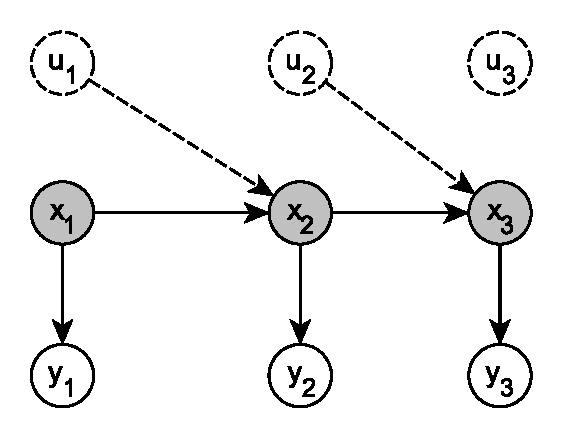
\includegraphics[scale=1.0]{linear_model.pdf}
\caption{Linear Graphical Model}
\label{fig_linmod}
\end{figure}
Intuitively, this model represents the situation where we are not sure about the state of the world but we have some idea represented by the prior $P(X_1)$. At each time step our state changes according to the transition function and we attempt to, amongst other things, infer the new state, perhaps given some observations related to the past and current state.

\subsection{Discrete Models}
In this section we briefly describe Markov Models because they link back to previous work done by the Chemical Engineering Department at the University of Pretoria. We focus on Hidden Markov Models for the remainder of the section because they generalise to Latent Linear Dynamical Systems. 

\subsubsection{Markov Models}
A first order Markov Model (sometimes called a Markov Chain) is shown in Figure \ref{fig_markov_chain}. Using the chain rule for Bayesian Networks we can immediately write down the joint probability distribution as shown in (\ref{eq_markov_chain_joint}).
\begin{equation}
P(X_{1:T}) = \Pi_{t=1}^T P(X_t|X_{t-1}) \text{ with } P(X_1|X_{-1}) = P(X_1)
\label{eq_markov_chain_joint}
\end{equation}  
\begin{figure}[H] 
\centering
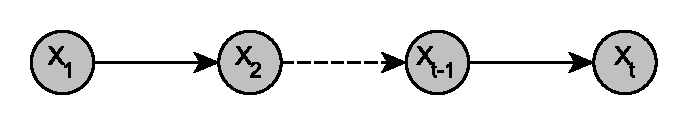
\includegraphics[scale=1.0]{markov_chain.pdf}
\caption{First Order Markov Chain}
\label{fig_markov_chain}
\end{figure}
This model describes the forward propagation of a discrete random variable through time. It is interesting to study the marginal distribution of $P(X_t)$ as it evolves through time. By d-separation we know that $X_t \indep X_{1:t-2} | X_t$. Thus, we only have to marginalise out the previous time step to compute the required distribution as shown in (\ref{eq_markov_chain_marg}).
\begin{equation}
P(X_t) = \sum_{x_{t-1}} P(X_t, x_{t-1}) = \sum_{x_{t-1}} P(x_{t-1})P(X_t|x_{t-1})
\label{eq_markov_chain_marg}
\end{equation}
Since we know that the transition function is a row stochastic $n \times n$ matrix (the random variable has $n$ discrete states) we can write (\ref{eq_markov_chain_marg}) in vector notation (\ref{eq_markov_chain_marg_vec}).
\begin{equation}
P(X_t) = \mathbf{p}_t = \mathbf{A}\mathbf{p}_{t-1} = \mathbf{M}^{t-1}\mathbf{p}_1
\label{eq_markov_chain_marg_vec}
\end{equation}
We have implicitly rewritten (\ref{eq_markov_chain_marg_vec}) in recursive format. Thus we have a recursive expression for the marginal distribution of $X$. If, as $t \rightarrow \infty$, we have that $\mathbf{p}_{t \rightarrow \infty} = \mathbf{p}_{\infty}$ is independent of $\mathbf{p}_1$ we call $\mathbf{p}_{\infty}$ the equilibrium distribution of the chain. 

We define the stationary distribution, in matrix notation, by (\ref{eq_markov_chain_stationary}).
\begin{equation}
\mathbf{p}_{\infty} = \mathbf{A}\mathbf{p}_{\infty}
\label{eq_markov_chain_stationary}
\end{equation}
Recalling the definition of the eigenvalue problem we see that the stationary distribution is just the eigenvector corresponding to the unit eigenvalue of $\mathbf{A}$. While this model may seem simplistic it is the foundation of Google's PageRank algorithm \cite{google}.  Intuitively $\mathbf{p}_\infty$ represents the steady state distribution of the random variable $X$ as it is propagated through time by the transition function $A$.

\subsubsection{Hidden Markov Models}
Hidden Markov Models extend Markov Models by incorporating the observed random variable $Y$ as shown in Figure \ref{fig_linmod}. At each time step it is now possible to observe some value $y_t$ which gives more information about the state of $X_t$. We are still in the setting of discrete random variables. It is not necessary to restrict $Y$ to be discrete but we do so for the sake of simplicity here. In later sections we will model hybrid and purely continuous systems. 

In general a Hidden Markov Model is just a specific case of the general Dynamic Bayesian Network class of graphical models. As such we already know that to fully specify the model we only require a prior state distribution $P(X_1)$, the transition probability function $P(X_t|X_{t-1})$, the observation or emission probability function $P(Y_t|X_t)$ and the Bayesian Network graphs of the initial time step and the next two time steps. We assume that the model's structure repeats at each time step and thus we only require the graph as shown in Figure \ref{fig_linmod}. 

We assume that the transition and observation probability functions are stationary. Consequently they may be represented by the row stochastic square matrices $P(x_t=i|x_{t-1}=j) = \mathbf{A}$ and $P(y_t=i|x_t=j) = \mathbf{B}$. Intuitively this means that the probability of state $x_{t-1}=j$ going to state $x_{t} = i$ is $A_{ij}$. Similarly, $B_{ij}$ is the probability of observing $y_t=i$ if the underlying state is $x_t=j$.

For the purposes of this dissertation we will always assume that the model parameters are known. In the previous section the four primary inference techniques were briefly mentioned. We now derive recursive expressions for each inference technique for discrete models of the form of Figure \ref{fig_linmod}. In the next section we show that these derivations also hold for the continuous case with some minor modifications.

\textbf{Filter:} $P(X_t|y_{1:t})$\\
We start the derivation by noting that $X_{t-1}$ d-separates $X_t$ from $X_{1:t-2}$. Thus $X_{t-1}$ contains all the hidden state information of the system up to and including $t-1$ - this is not surprising since we have assumed a first order Markov system. This is why we consider the reduced state joint $P(X_t, X_{t-1},y_{1:t})$.
\begin{equation}
\begin{aligned}
P(X_t, y_{1:t}) &= \sum_{x_{t-1}} P(X_t, x_{t-1}, v_{1:t-1},v_t)\\
&= \sum_{x_{t-1}} P(y_{1:t-1}, x_{t-1})P(X_t, y_t|y_{1:t}, x_{t-1})\\  & = \sum_{x_{t-1}} P(y_{1:t-1}, x_{t-1})P(X_t|y_{1:t}, x_{t-1})P(y_t|X_t,y_{1:t}, x_{t-1}) \\
&= \sum_{x_{t-1}} P(y_{1:t-1}, x_{t-1})P(X_t|x_{t-1})P(y_t|X_t) \\
\end{aligned}
\label{eq_forward_no_recur}
\end{equation}
Where the expansions followed from the chain rule and the cancellations followed from the conditional independence assumptions of the transition and observation functions. Now we define $\alpha(X_t) \equiv P(X_t,y_{1:t})$. Then (\ref{eq_forward_recur}) follows from (\ref{eq_forward_no_recur}).
\begin{equation}
\begin{aligned}
&\alpha(X_t) = P(y_t|X_t)\sum_{x_{t-1}}P(X_t|X_{t-1})\alpha(X_{t-1}) \text{ for } t>1\\
&\text{with } \alpha(X_1) = P(X_1, y_1) = P(X_1)P(y_1|X_1)
\end{aligned}
\label{eq_forward_recur}
\end{equation}
Clearly we have just derived a recursive expression for the joint distribution $P(X_t, y_{1:t})$. This recursion is called forward recursion in graphical model literature \cite{barber}. To complete our task of estimating $P(X_t|y_{1:t})$ we recall Bayes' Theorem as shown in (\ref{eq_forward_filter}).
\begin{equation}
P(X_t|y_{1:t}) = \frac{P(X_t, y_{1:t})}{P(y_{1:t})} = \frac{\alpha(X_t)}{P(y_{1:t})}
\label{eq_forward_filter}
\end{equation}
Noting that $P(y_{1:t})$ is just a normalisation constant it suffices to normalise $\alpha(X_t)$ to find the filtered distribution of $X_t$ given the observations $y_{1:t})$. One often uses logarithms to perform the filter calculations as machine precision errors become a problem for large $t$ due to the multiplication of small fractions \cite{barber}.

\textbf{Smoothing:} $P(X_t|y_{1:T})$ for $t<T$\\
The smoothing algorithm we study here is called the parallel smoothing algorithm. The recursion expression we derive first is often called the Backwards algorithm in literature \cite{murphy1}.

We start by splitting the joint $P(X_t, y_{1:T}) = P(X_t, y_{1:t})P(y_{t+1:T}|X_t,y_{1:t})$ by the chain rule and using d-separation to reduce it further $P(X_t, y_{1:T}) = P(X_t, y_{1:t})P(y_{t+1:T}|X_t) = \alpha(X_t)\beta(X_t)$. Effectively the last step implies that future observations are independent of past observations given the current state. We have defined $\beta(X_t)\equiv P(y_{t+1:T}|X_t)$ and continue the derivation in (\ref{eq_backwards_no_recur}).
\begin{equation}
\begin{aligned}
P(y_{t:T}|X_{t-1}) &= \sum_{x_t} P(y_t, y_{t+1:T}, x_t|X_{t-1}) \\
&= \sum_{x_t} P(y_{t+1:T}, x_t | X_{t-1})P(y_t| y_{t+1:T}, x_t, X_{t-1}) \\
&= \sum_{x_t} P(y_{t+1:T}, x_t | X_{t-1})P(y_t| x_t) \\
&= \sum_{x_t} P(x_t | X_{t-1})P(y_{t+1:T}| x_t,X_{t-1})P(y_t| x_t) \\
&= \sum_{x_t} P(x_t | X_{t-1})P(y_{t+1:T}| x_t)P(y_t| x_t) \\
\end{aligned}
\label{eq_backwards_no_recur}
\end{equation}
We have made judicious use of the implied independence assertions (via d-separation) of Figure \ref{fig_linmod}. Making use of the definition of $\beta$ we have (\ref{eq_backwards_recur}).
\begin{equation}
\begin{aligned}
&\beta(X_{t-1}) = \sum_{x_t} P(x_t | X_{t-1})\beta(x_t)P(y_t| x_t) \text{ for } 2 \leq t \leq T \\
&\text{with } \beta(X_T) = \mathbf{1}
\end{aligned}
\label{eq_backwards_recur}
\end{equation}
The recursion initial condition $\beta(X_T) = 1$ stems from Bayes' Theorem and the definition of $\alpha$ as shown in (\ref{eq_backwards_recur_initial}).
\begin{equation}
\begin{aligned}
P(X_t|y_{1:T}) &= \frac{P(X_t, y_{1:T})}{P(y_{1:T})} \\
&= \frac{\alpha(X_t)\beta(X_t)}{P(y_{1:T})}\\
&= \frac{P(X_t, y_{1:T})\beta(X_t)}{P(y_{1:T})}\\
&\implies \beta(X_T) = \mathbf{1}
\end{aligned}
\label{eq_backwards_recur_initial}
\end{equation}
The smoothed posterior is given by applying Bayes' Theorem as shown in (\ref{eq_smooth}).
\begin{equation}
P(X_t|y_{1:T}) = \frac{\alpha(X_t)\beta(X_t)}{\sum_{x_t}\alpha(x_t)\beta(x_t)}
\label{eq_smooth}
\end{equation}
Together the $\alpha - \beta$ recursions are called the Forwards-Backwards algorithm and find extensive use in general purpose inference of Dynamic Bayesian Networks \cite{murphy1}.

Numerical issues may also become problematic due to the multiplication of small positive numbers. In practice it is often necessary to work in the log space to attenuate these problems \cite{barber}. 

\textbf{Viterbi Decoding:} $x_{1:T}^* = \underset{x_{1:T}}{\text{arg max }} P(x_{1:T}|y_{1:T})$ \\
In Viterbi decoding, or finding the most likely sequence of states which best describe the observations, one attempts to find the sequence of $x_{1:T}$ such that the joint probability function $P(x_{1:T}, y_{1:T})$ is maximised. This is equivalent to finding $ \underset{x_{1:T}}{\text{arg max }} P(x_{1:T}|y_{1:T})$ because, if one uses the chain rule on the joint, the observations will just be a constant factor. 

Intuitively we first attempt to find the maximum of the joint and then determine which sequence of states led to this maximal joint. By using the chain rule for Bayesian Networks we can rewrite the joint maximisation problem as in (\ref{eq_viterbi_joint}).
\begin{equation}
\begin{aligned}
\underset{x_{1:T}}{\text{max }} P(x_{1:T}, y_{1:T}) &= \underset{x_{1:T}}{\text{max }} \Pi_{t=1}^T P(y_t|x_t) P(x_t|x_{t-1})\\
&= \left(\underset{x_{1:T-1}}{\text{max }} \Pi_{t=1}^{T-1} P(y_t|x_t) P(x_t|x_{t-1}) \right) \underset{x_{T}}{\text{max }} P(y_T|x_T) P(x_T|x_{T-1})
\end{aligned}
\label{eq_viterbi_joint}
\end{equation}
Defining $\mu(X_{t-1}) \equiv \underset{x_{t}}{\text{max }} P(y_t|x_t) P(x_t|x_{t-1})$ we can rewrite (\ref{eq_viterbi_joint}) as (\ref{eq_viterbi_max_factor_mu}).
\begin{equation}
\underset{x_{1:T}}{\text{max }} P(x_{1:T}, y_{1:T}) =\underset{x_{1:T-1}}{\text{max }} \Pi_{t=1}^{T-1} P(y_t|x_t) P(x_t|x_{t-1}) \mu(x_{T-1})
\label{eq_viterbi_max_factor_mu}
\end{equation}
Thus we have a recursive expression to find the value of the joint under the most likely sequence of states given the observations as shown in (\ref{eq_viterbi_recur}).
\begin{equation}
\begin{aligned}
&\mu(x_{t-1}) = \underset{x_{t}}{\text{max }} P(y_t|x_t) P(x_t|x_{t-1}) \mu(x_t) \text{ for } 2 \leq t \leq T \\
&\text{with } \mu(x_T) = 1 
\end{aligned}
\label{eq_viterbi_recur}
\end{equation}
The recursive expression in (\ref{eq_viterbi_recur}) implies that the effect of maximising over over the previous time step can be compressed into a message (a function) of the current time step. Effectively we pass theses messages backward in time to find the maximum joint in terms of $x_1$. We then find the state which maximises this joint and pass this message forward.  Continuing in this way, we have (\ref{eq_viterbi_recur_forward}).
\begin{equation}
\begin{aligned}
x_1^* &= \underset{x_{1}}{\text{arg max }}P(y_1|x_1)P(x_1)\mu(x_1) \\
x_2^* &= \underset{x_{2}}{\text{arg max }}P(y_2|x_2)P(x_2|x_1^*)\mu(x_2) \\
&~~\vdots \\
x_t^* &= \underset{x_{t}}{\text{arg max }}P(y_t|x_t)P(x_t|x_{t-1}^*)\mu(x_t)
\end{aligned}
\label{eq_viterbi_recur_forward}
\end{equation}
This algorithm is called the Viterbi algorithm. It is computationally efficient since the optimisations occur only on a single variable.

\textbf{Prediction:} $P(X_{t+1}|y_{1:t})$ and $P(Y_{t+1}|y_{1:t})$  \\
The one step ahead prediction expression for both the states and observations is derived here. We again start by noticing that given all the observations  up to time $t$ the current state d-separates  all previous states. Thus, to infer information about the next state we only need to marginalise out the current state $X_t$. Furthermore, the next state d-separates the next observation from all the previous states. Thus, to infer information about the next observation we additionally only need to marginalise out $X_{t+1}$.

We start with predicting the next state distribution. We have applied the chain rule, the independence assertions and used the definition of $\alpha$ to derive (\ref{eq_prediction_state}).
\begin{equation}
\begin{aligned}
P(X_{t+1}|y_{1:t}) &= \sum_{x_t} P(X_{t+1}, x_t|y_{1:t}) \\
&= \sum_{x_t} P(x_t|y_{1:t})P(X_{t+1}|x_t, y_{1:t}) \\
&= \sum_{x_t} P(x_t|y_{1:t})P(X_{t+1}|x_t) \\
&= \sum_{x_t} \alpha(x_t)P(X_{t+1}|x_t) \\
\end{aligned}
\label{eq_prediction_state}
\end{equation}
Clearly the state prediction uses the filtered state estimate and projects that forward using the transition function.

Next we derive the observation prediction. Again we apply the chain rule, use the independence assertions and use the definition of $\alpha$ to derive (\ref{eq_prediction_observation}).
\begin{equation}
\begin{aligned}
P(Y_{t+1}|y_{1:t}) &= \sum_{x_t, x_{t+1}} P(x_{t+1}, x_t, Y_{t+1}|y_{1:t})\\
&= \sum_{x_t, x_{t+1}} P(x_t|y_{1:t})P(x_{t+1}, Y_{t+1}|y_{1:t}, x_t) \\
&= \sum_{x_t, x_{t+1}} P(x_t|y_{1:t})P(x_{t+1}|y_{1:t}, x_t)P(Y_{t+1}|y_{1:t}, x_t, x_{t+1}) \\
&= \sum_{x_t, x_{t+1}} P(x_t|y_{1:t})P(x_{t+1}|x_t)P(Y_{t+1}|x_{t+1}) \\
&= \sum_{x_t, x_{t+1}} \alpha(x_t)P(x_{t+1}|x_t)P(Y_{t+1}|x_{t+1}) \\
\end{aligned}
\label{eq_prediction_observation}
\end{equation}
Clearly the observation prediction is just an extension of the state prediction. We effectively just predict the next state and use the observation function to predict the observation distribution.

It is pleasing that the prediction expressions are closely related to each other and effectively only depend on the filtered state estimate and the transition or observation functions.

\textbf{Burglar Localisation Problem} \\
We have taken the time to derive each inference algorithm and thus it is desirable to conduct a numerical experiment. The type of problem we consider here is a localisation problem. This type of problem (and its extensions) has many applications in robotics and object tracking.

The problem is taken from Chapter 23 in Barber's book \textit{Bayesian Reasoning and Machine Learning} \cite{barber}. Briefly, it is necessary to infer the location of a burglar in your house given observations (noises) you perceive from an adjoining room. You discretise the room the burglar is in into $n^2$ blocks. Each block in the square room is a hidden state. You observe two distinct types of noises: creaks and bumps. From the knowledge of your house you know which blocks are likely to creak and which are likely to bump if the burglar is on that block. This is shown in Figure \ref{fig_burlgar_observations}: a dark block indicates it is likely to emit a noise with probility 0.9 and a light block with probability 0.01. The noises are independent of each other.
\begin{figure}[H] 
\centering
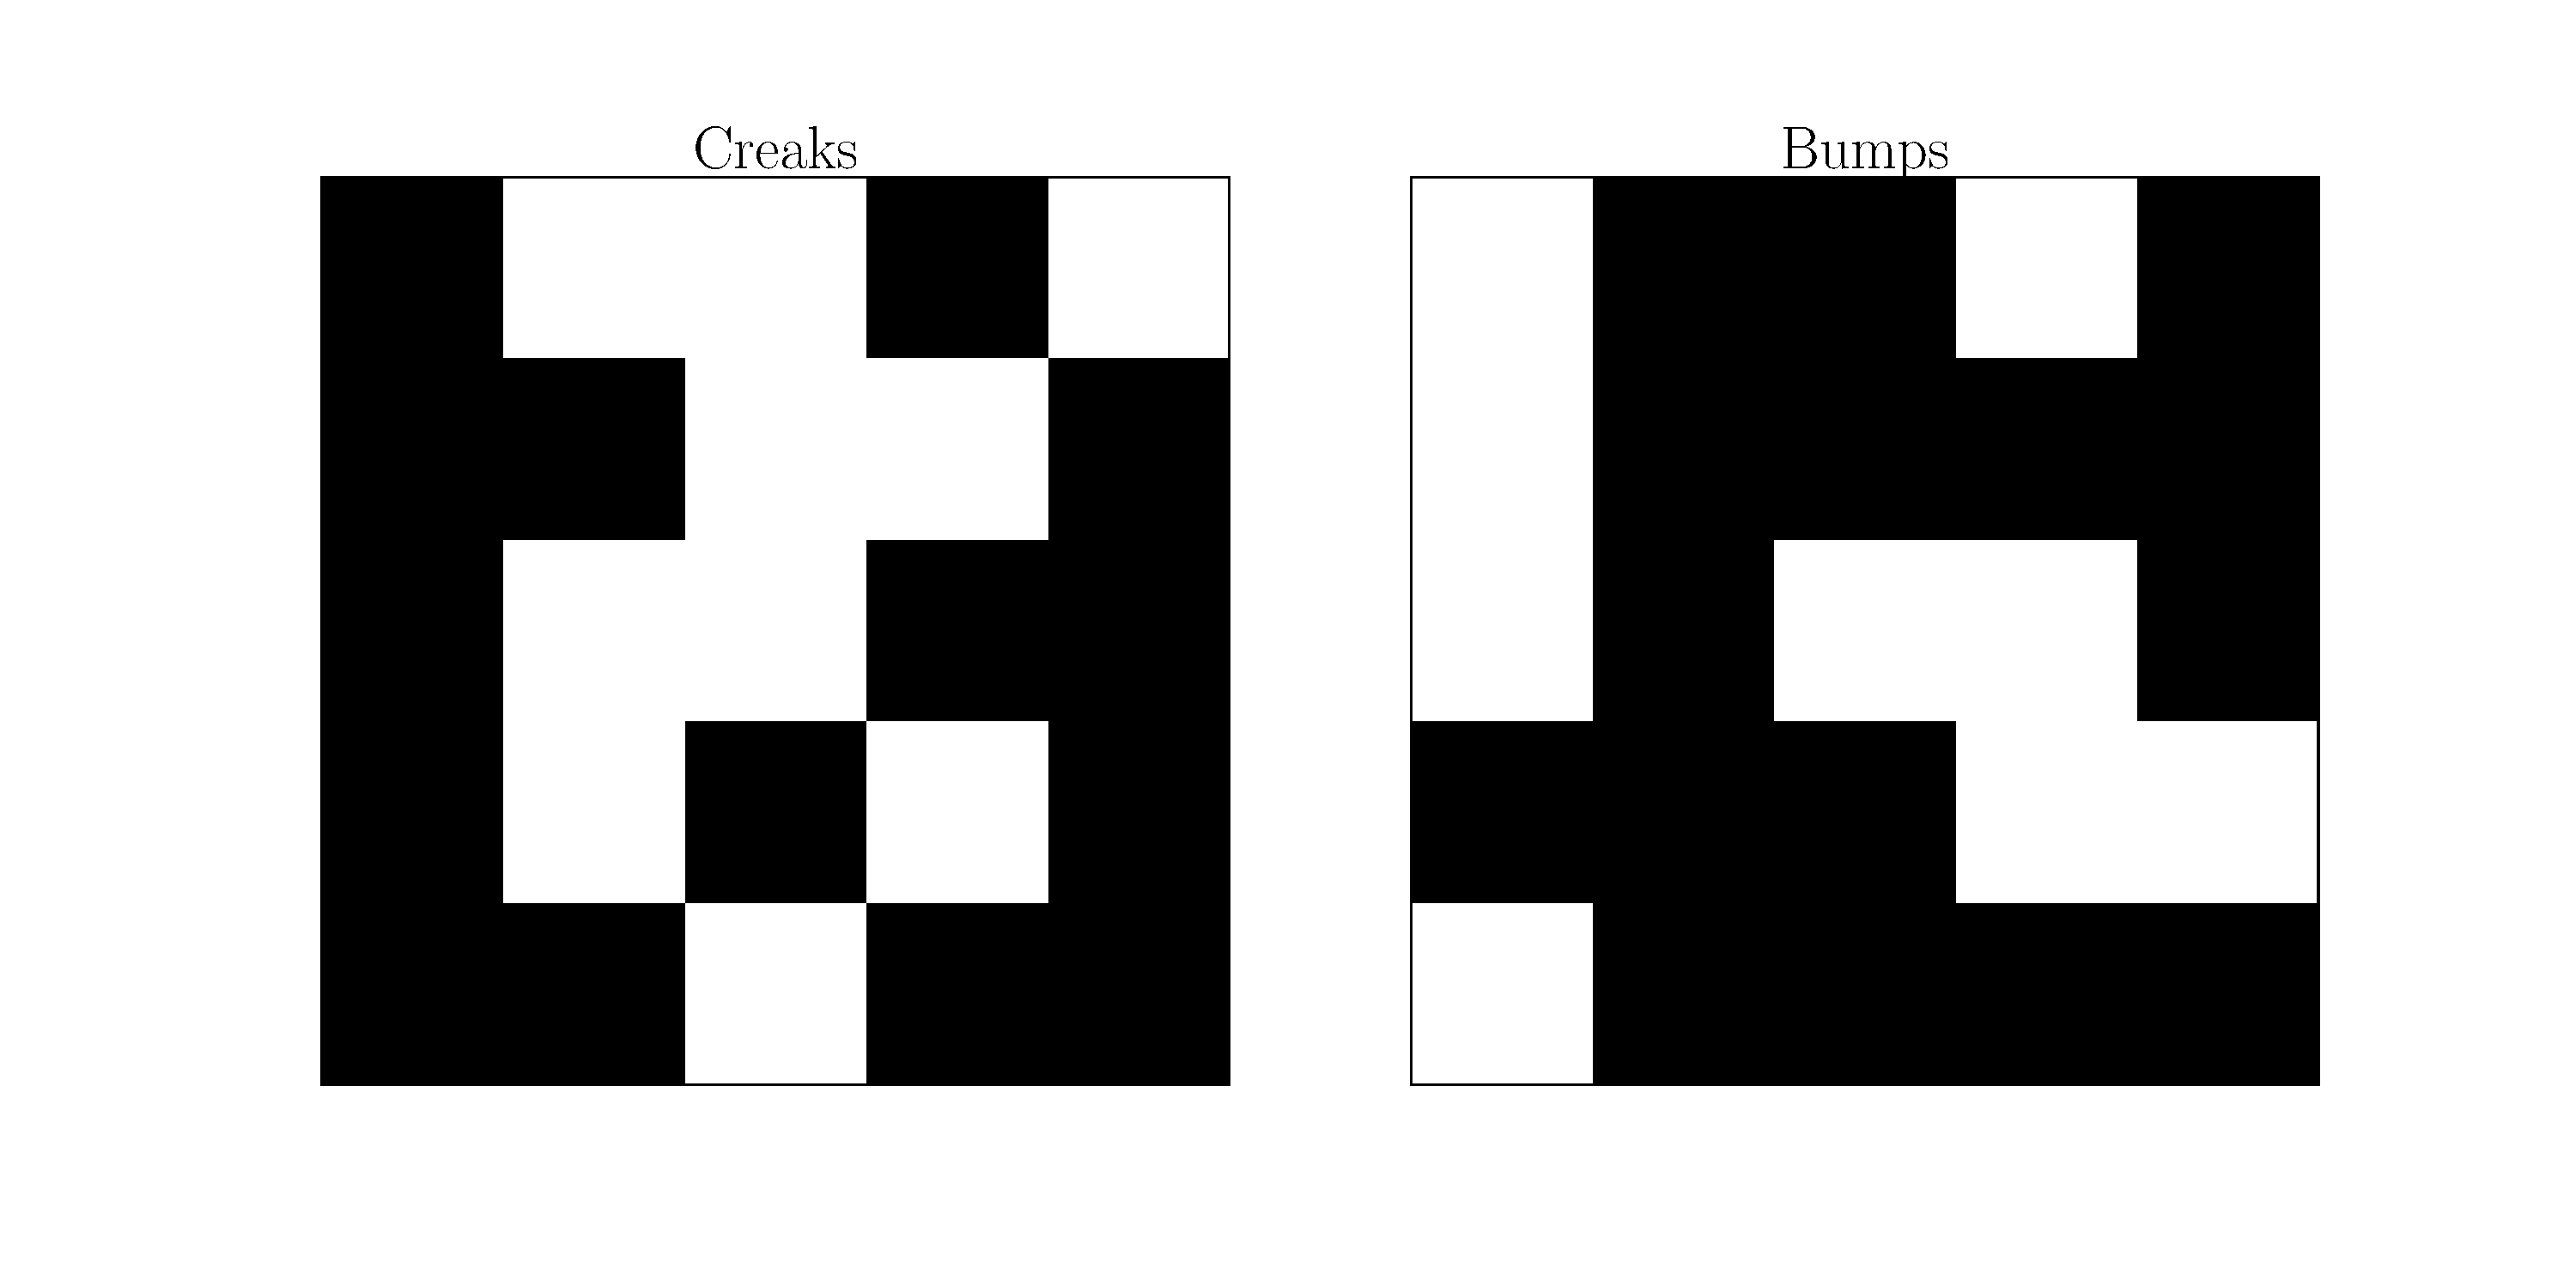
\includegraphics[scale=0.20]{burglar_observations.pdf}
\caption{Burglar Problem Observations}
\label{fig_burlgar_observations}
\end{figure}
The burglar moves up, down, left and right with equal probability where appropriate. See Barber for more details on the example. It is necessary to perform inference to determine the path of the burglar both in real time and with the benefit of hindsight. Applying the inference techniques we developed earlier results in Figure \ref{fig_burglar_inference}. 
\begin{figure}[H] 
\centering
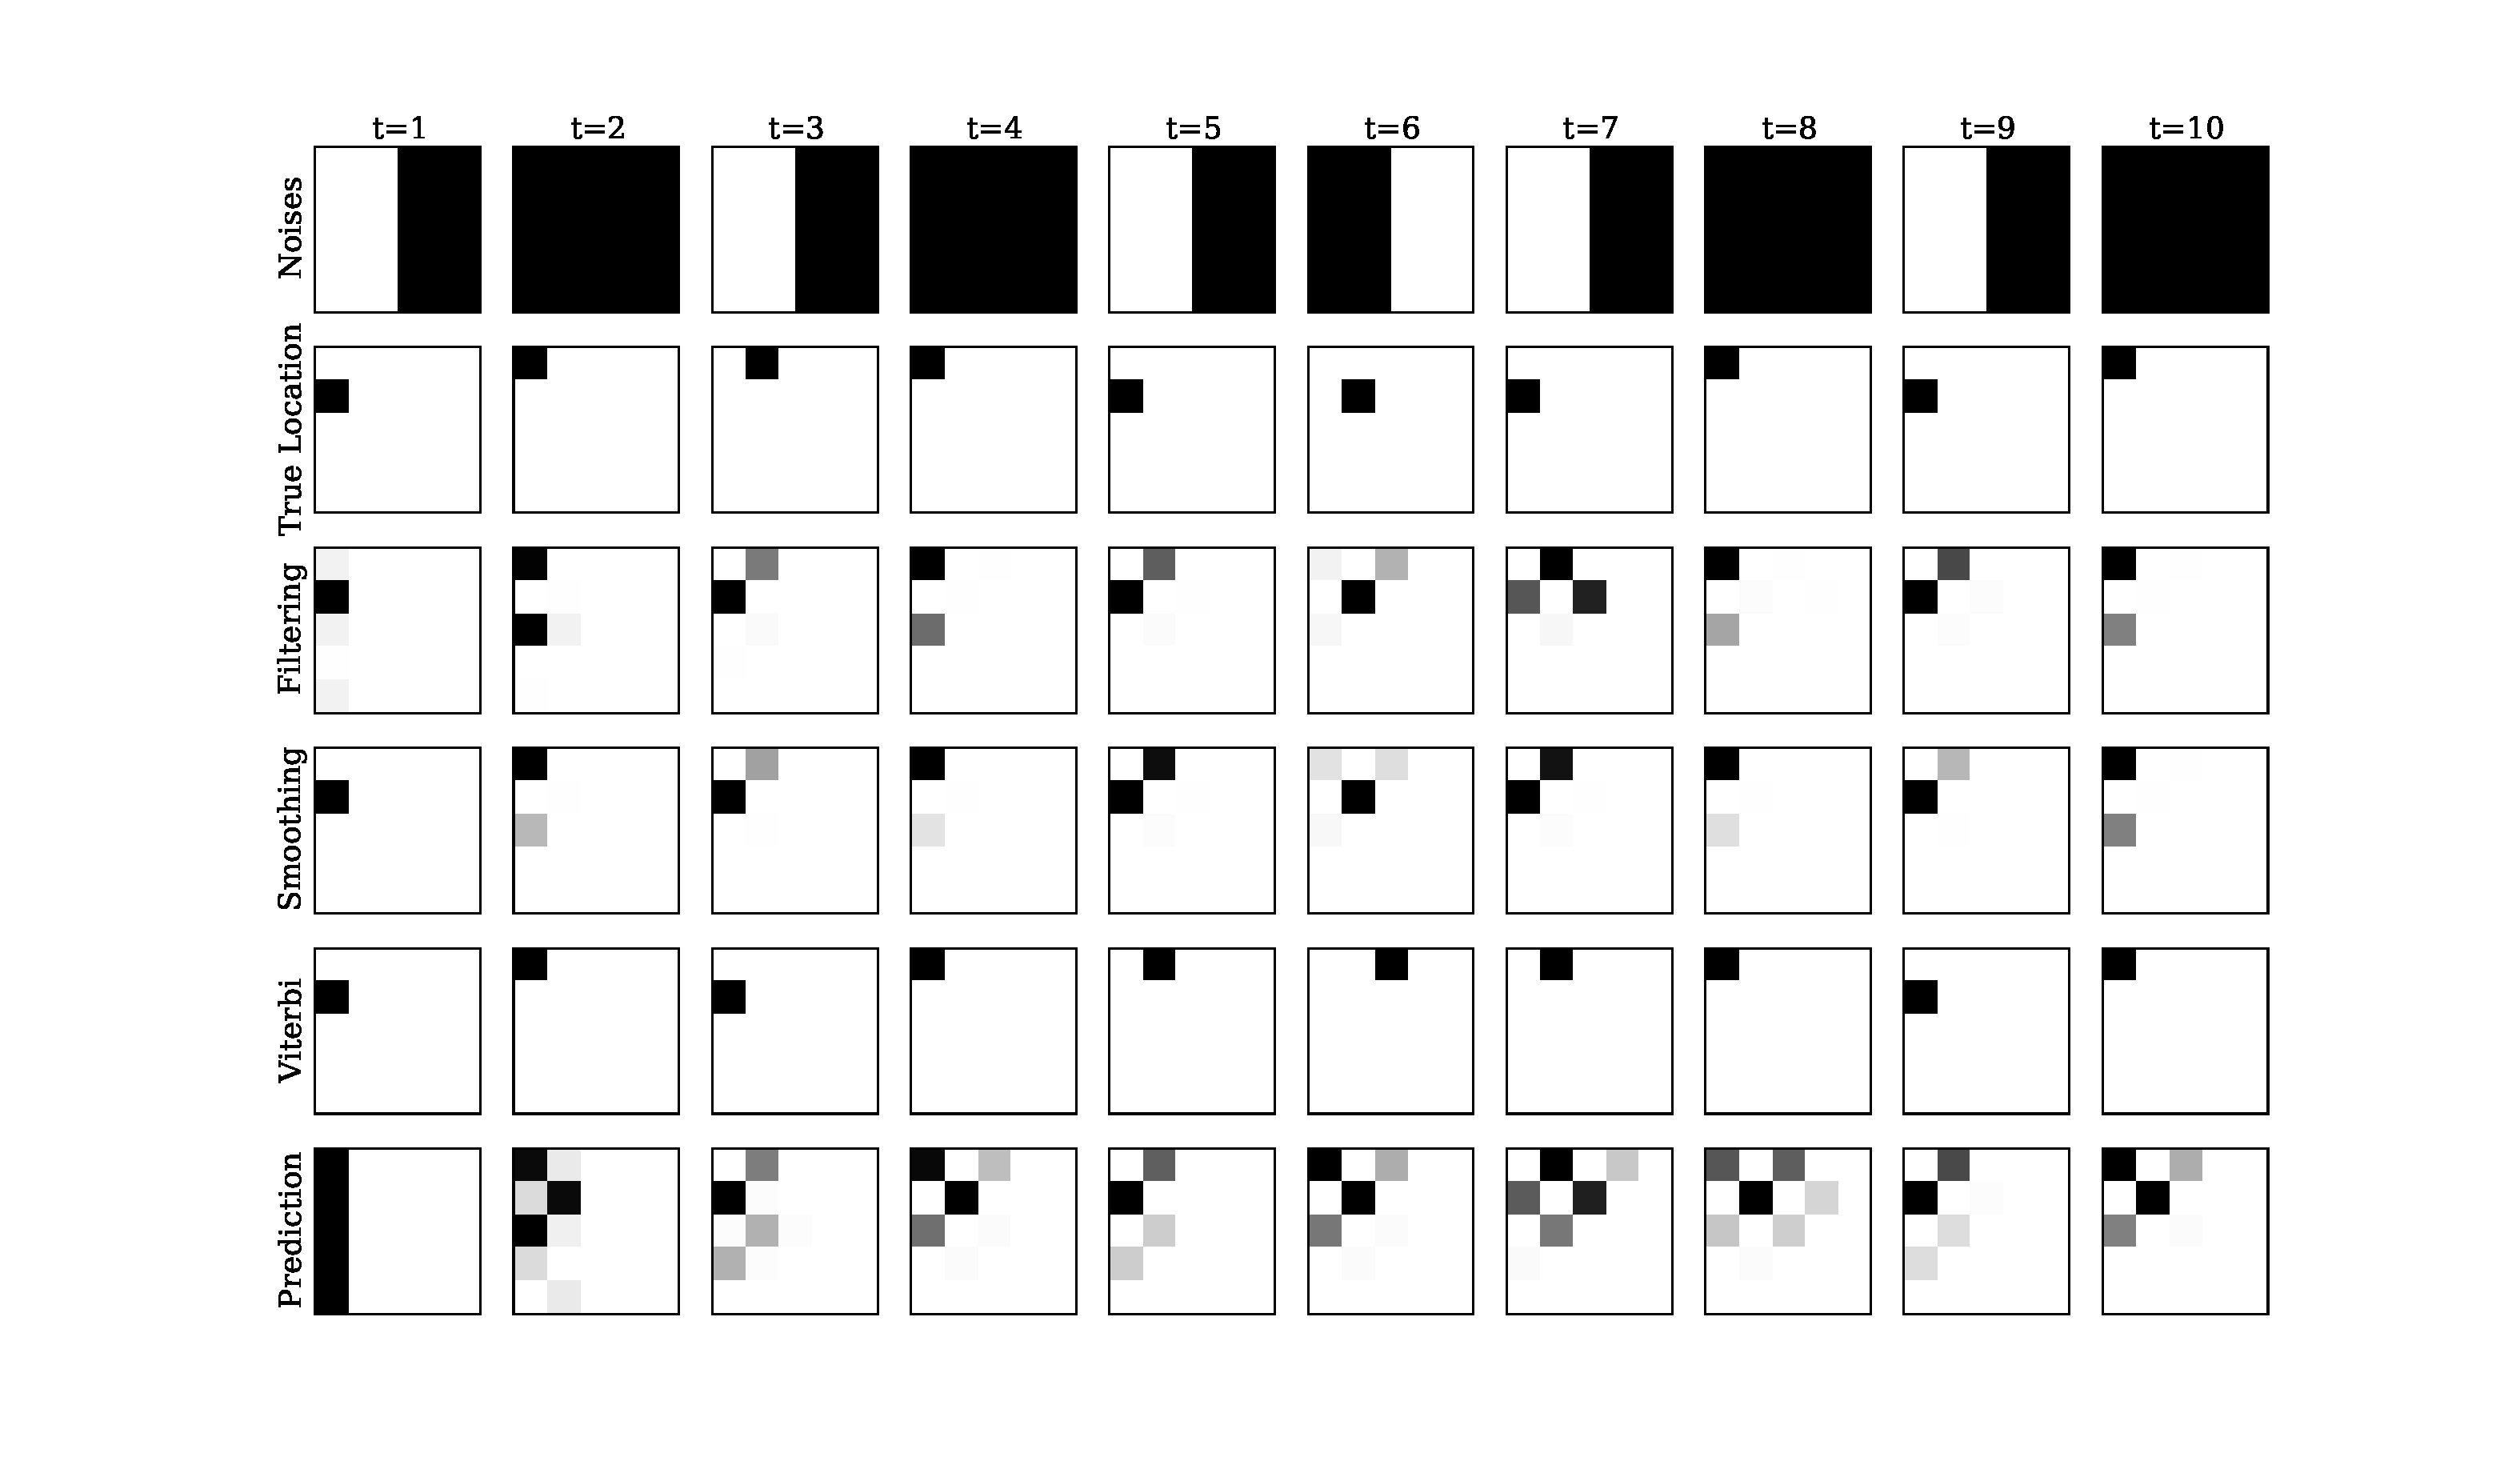
\includegraphics[scale=0.29]{burglar_inference.pdf}
\caption{Burglar Problem: Filter, Smoothing, Viterbi Decoding and Prediction}
\label{fig_burglar_inference}
\end{figure}
In this context filtering means we estimate the location of the burglar given all the past observations at the current time step. This inference can be done on-line. Smoothing means we attempt to estimate his position with hindsight given all the observations starting from the first time step and moving forwards. In Viterbi decoding we attempt to estimate the most likely path path of the burglar. Finally the prediction algorithm is self-explanatory.

It is interesting to note that smoothed posterior converges to the filtered posterior near the end of the time window. Reflecting on the expression for smoothing this is not surprising since at $t=T$ the smoothing component of the Forwards-Backwards algorithm is unity. It is also interesting to note that the prediction algorithm is very much dependent on the quality of the transition function. The four block pattern readily apparent in the prediction distribution originates from the transition function (the burglar is equally likely to move in any direction). This strongly implies that the closer the transition function is to reality the better our predictions will be. 

Hidden Markov Models are very powerful and have found many uses e.g. speech recognition, object tracking and bio-informatics \cite{barber}. Many extensions of the basic model (see Figure \ref{fig_linmod}) exist which are much more expressive. However, we are interested in modelling and reasoning about continuous random variables. For such applications the Hidden Markov Model, due to the discrete assumption, is inappropriate. Fortunately, the techniques investigated in this section carry over to the continuous case as we will see next.  

\subsection{Continuous Models}
In the previous section we developed inference algorithms but assumed that the transition and observation functions were discrete. We also noted that this assumption is not appropriate for continuous data. The reason is that one would invariably need to discretise the state domain and this would result in an intractably large state space if one requires reasonable resolution. To address this issue we extend the previous model to include both continuous states and observations. 

We assume linearity and that all the distributions are Gaussian. While these are strong assumptions they form the building blocks of much more expressive models as we will discover in the next section. 

%\bibliographystyle{plain}
%\bibliography{research}

\end{document}